\begin{figure}[ht!]
\centering
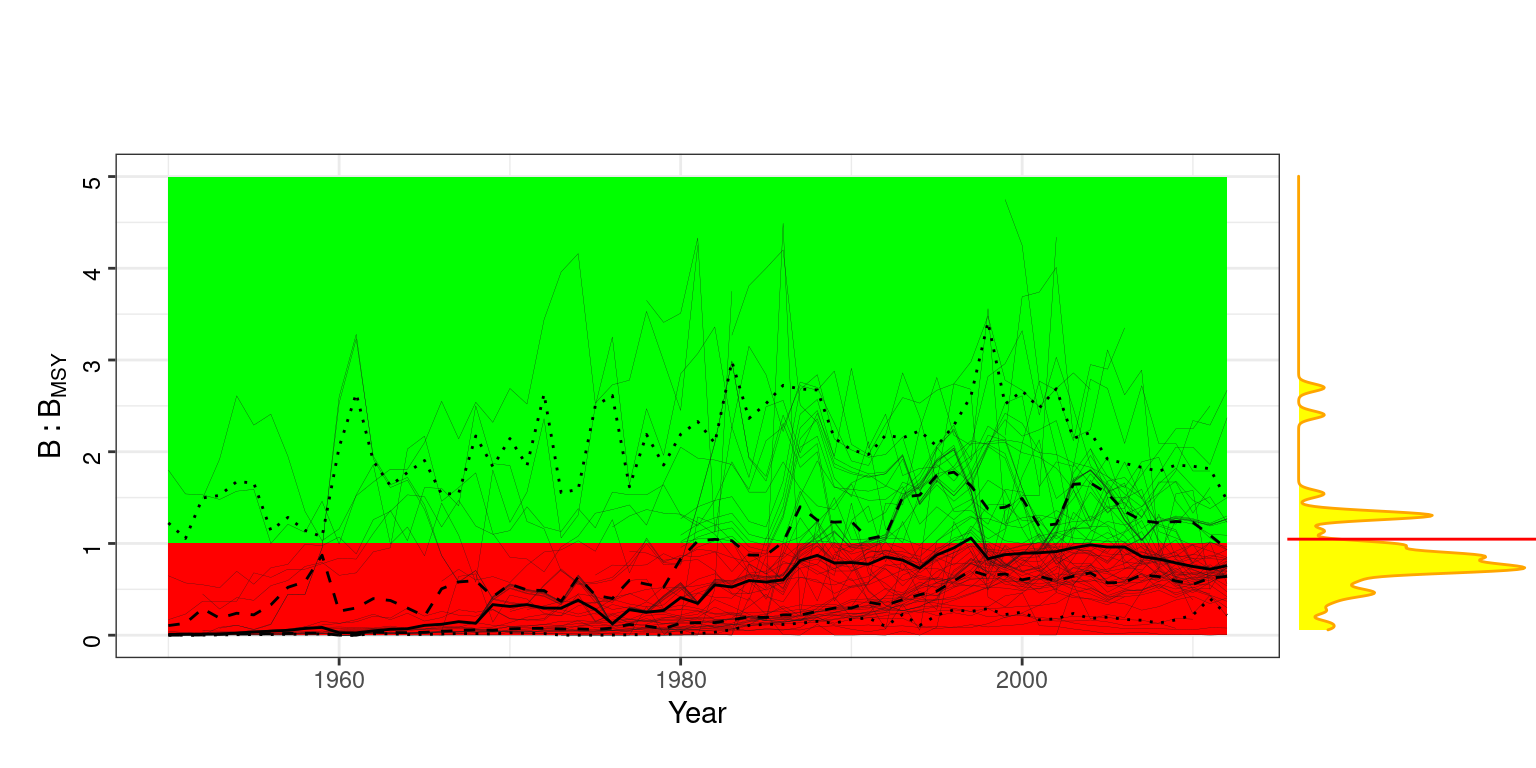
\includegraphics[width=0.75\textwidth]{figs/ts-f-1.png}
\caption{Time series of $F:F_{MSY}$ for the RAM Legacy database assessments.}
\label{fig:ts-f}
\end{figure}

\begin{figure}[ht!]
\centering
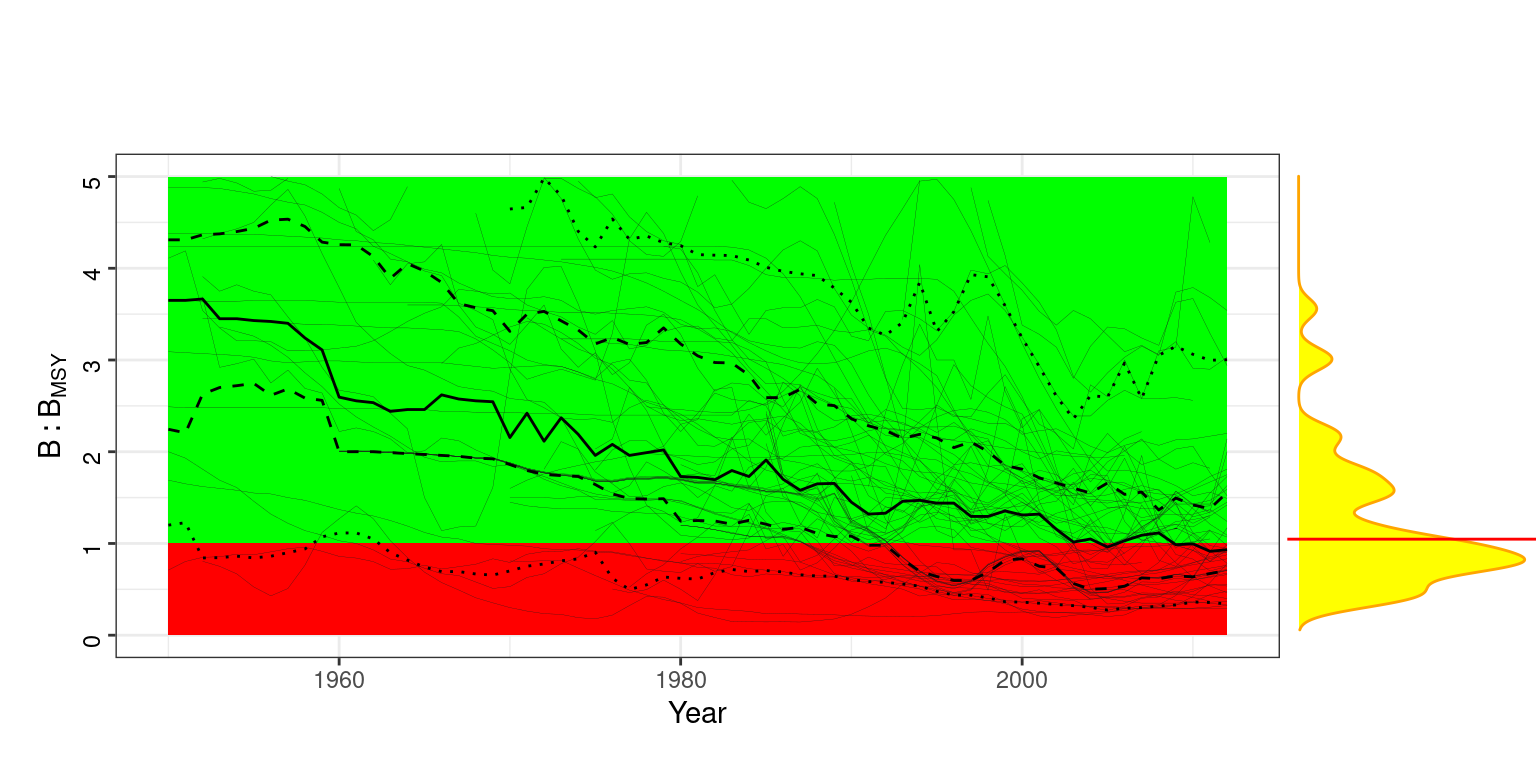
\includegraphics[width=0.75\textwidth]{figs/ts-ssb-1.png}
\caption{Time series of $B:B_{MSY}$ for the RAM Legacy database assessments.}
\label{fig:ts-s}
\end{figure}

\begin{figure}[ht!]
\centering
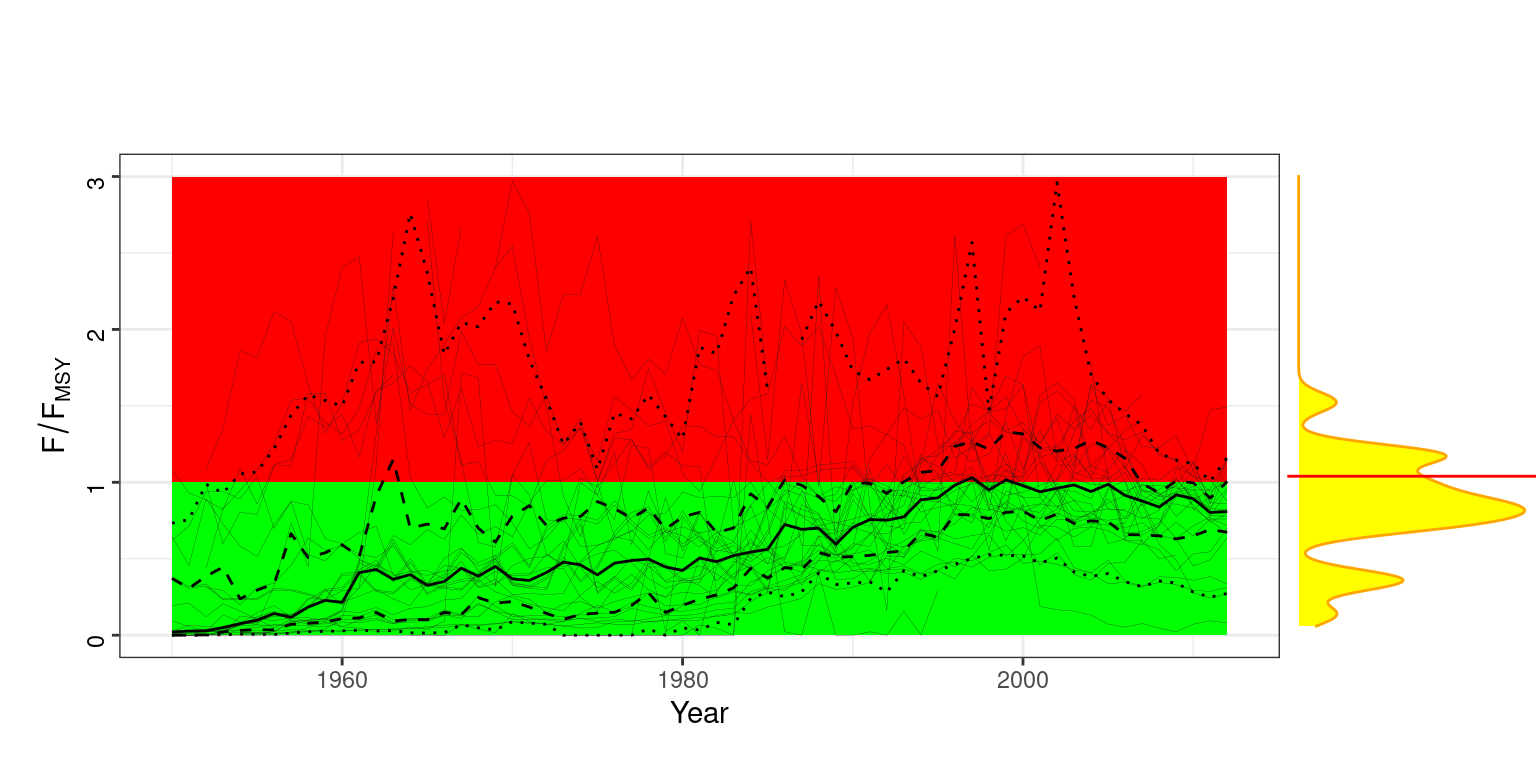
\includegraphics[width=0.75\textwidth]{figs/ts-c-1.png}
\caption{Time series of $Catch:MSY$ for the RAM Legacy database assessments.}
\label{fig:ts-c}
\end{figure}

\begin{figure}[ht!]
\centering
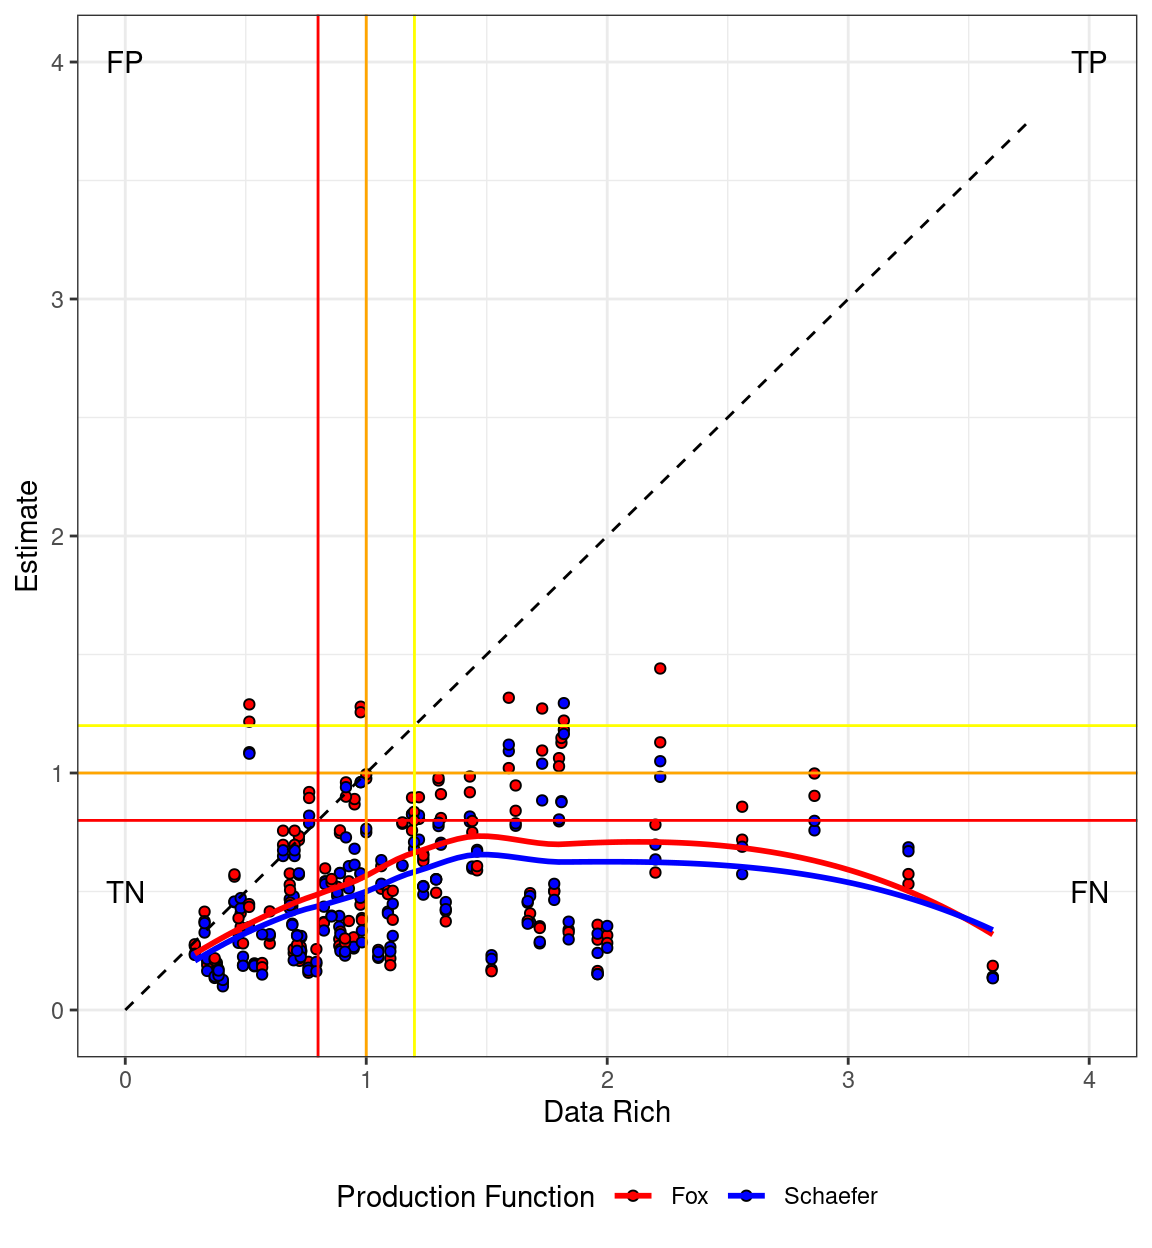
\includegraphics[width=0.75\textwidth]{figs/cf-jabba-1.png}
\caption{Comparisons of $B:B_{MSY}$, If the COM was unbiased y=x, if COM was biased but tunable then the smoother should be linear.}
\label{fig:cf-com}
\end{figure}

\begin{figure}[ht!]
\centering
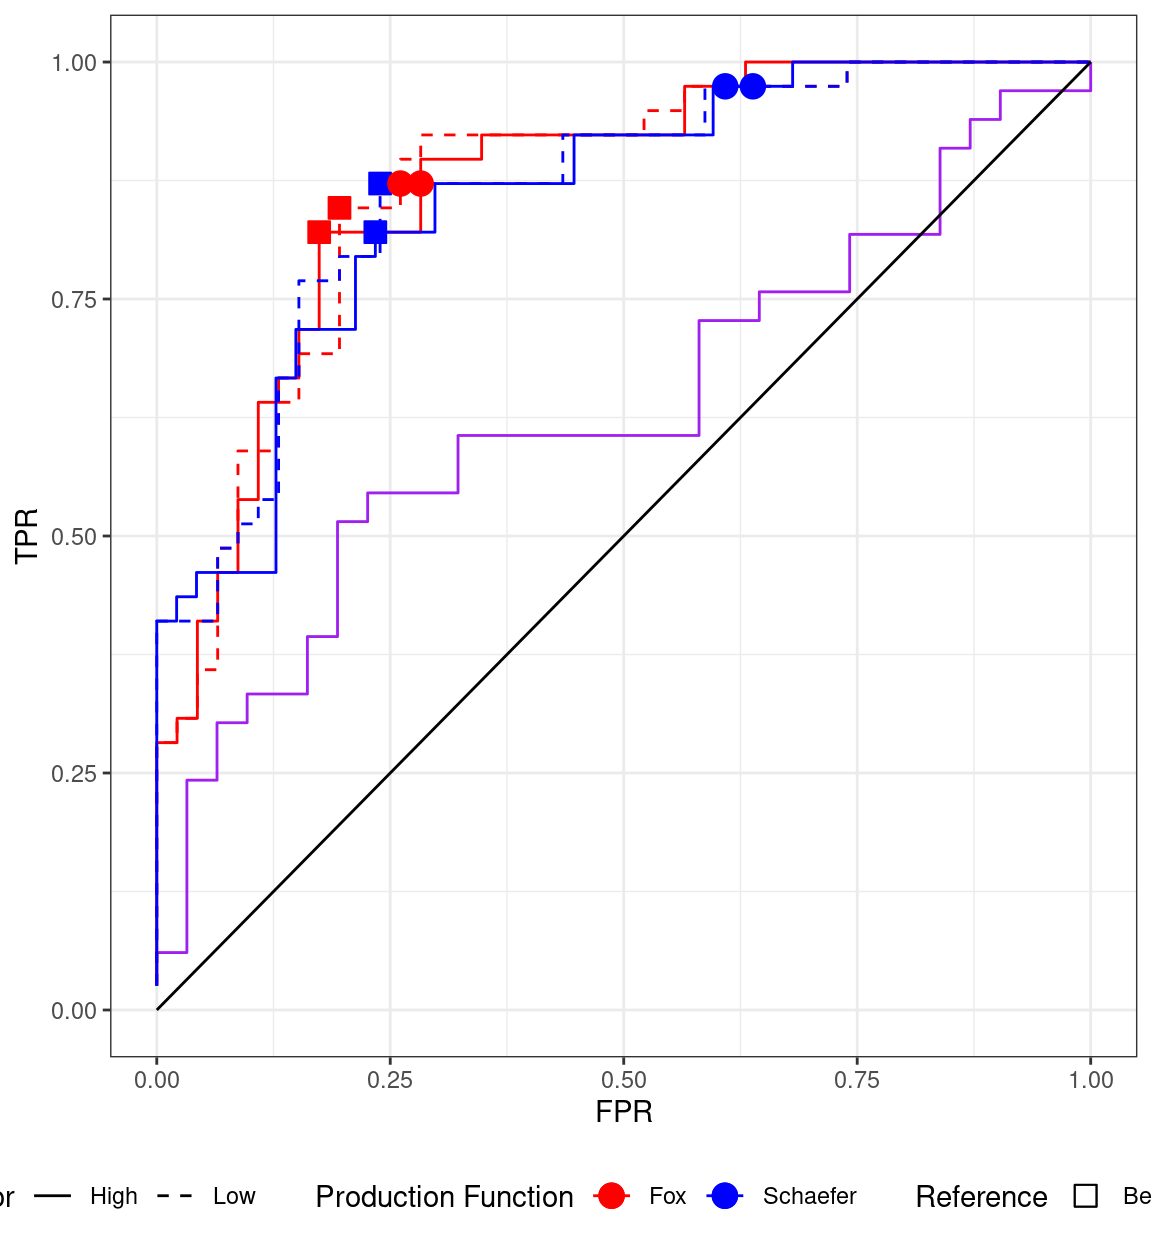
\includegraphics[width=0.75\textwidth]{figs/roc-jabba-1.png}
\caption{ROC curves for COMs.}
\label{fig:roc-com}
\end{figure}

\begin{figure}[ht!]
\centering
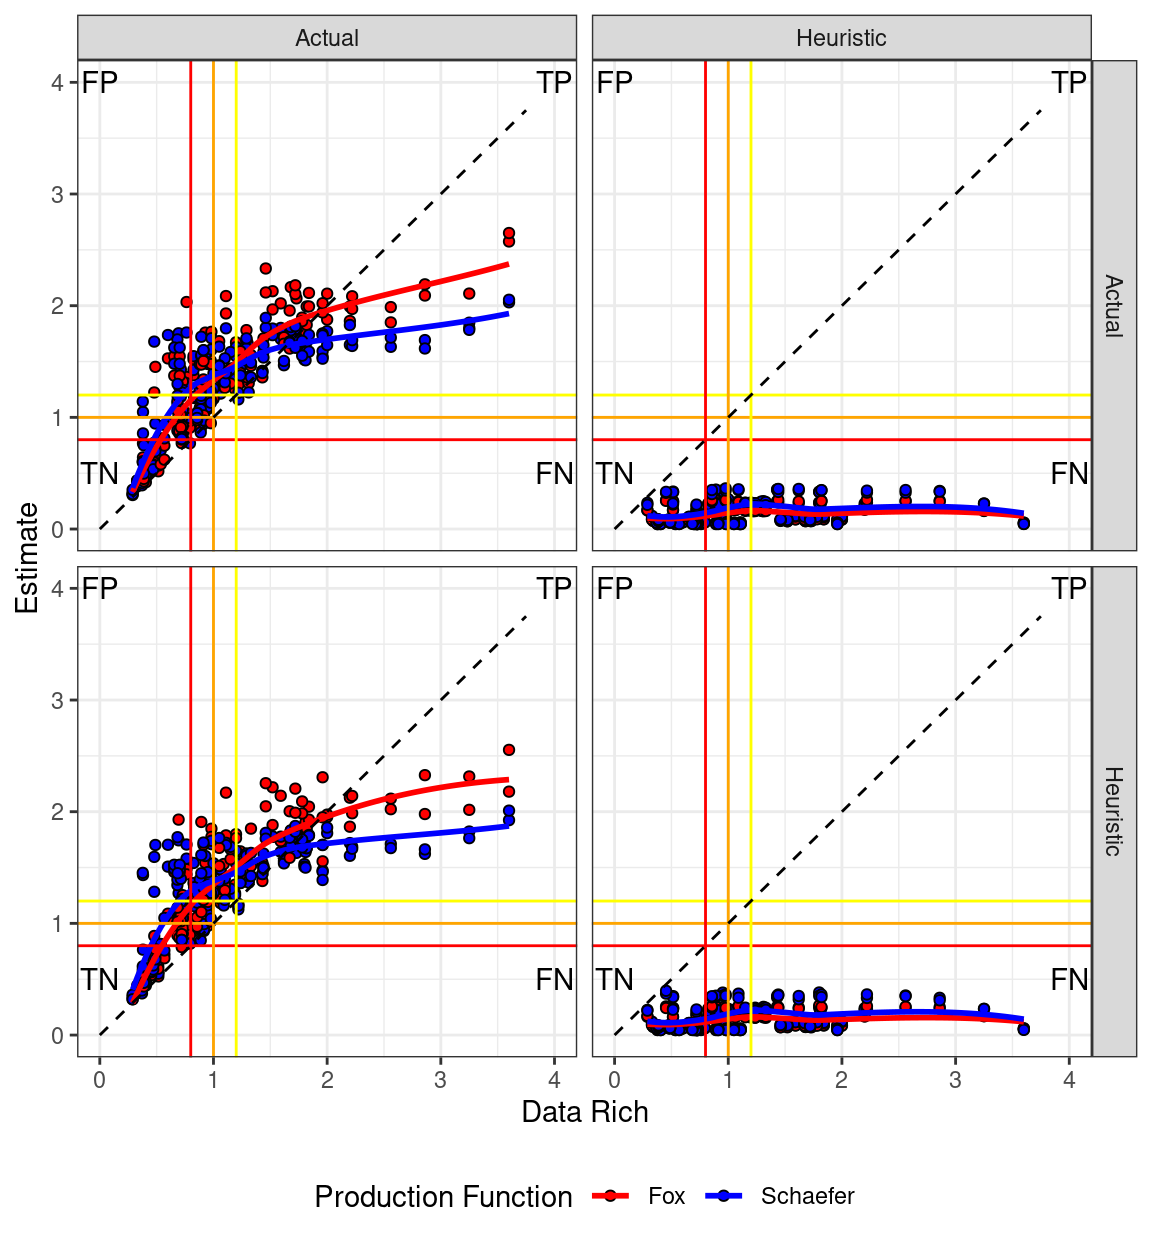
\includegraphics[width=0.75\textwidth]{figs/cf-1.png}
\caption{Comparisons of $B:B_{MSY}$, If the COM was unbiased y=x, if COM was biased but tunable then the smoother should be linear.}
\label{fig:cf}
\end{figure}

\begin{figure}[ht!]
\centering
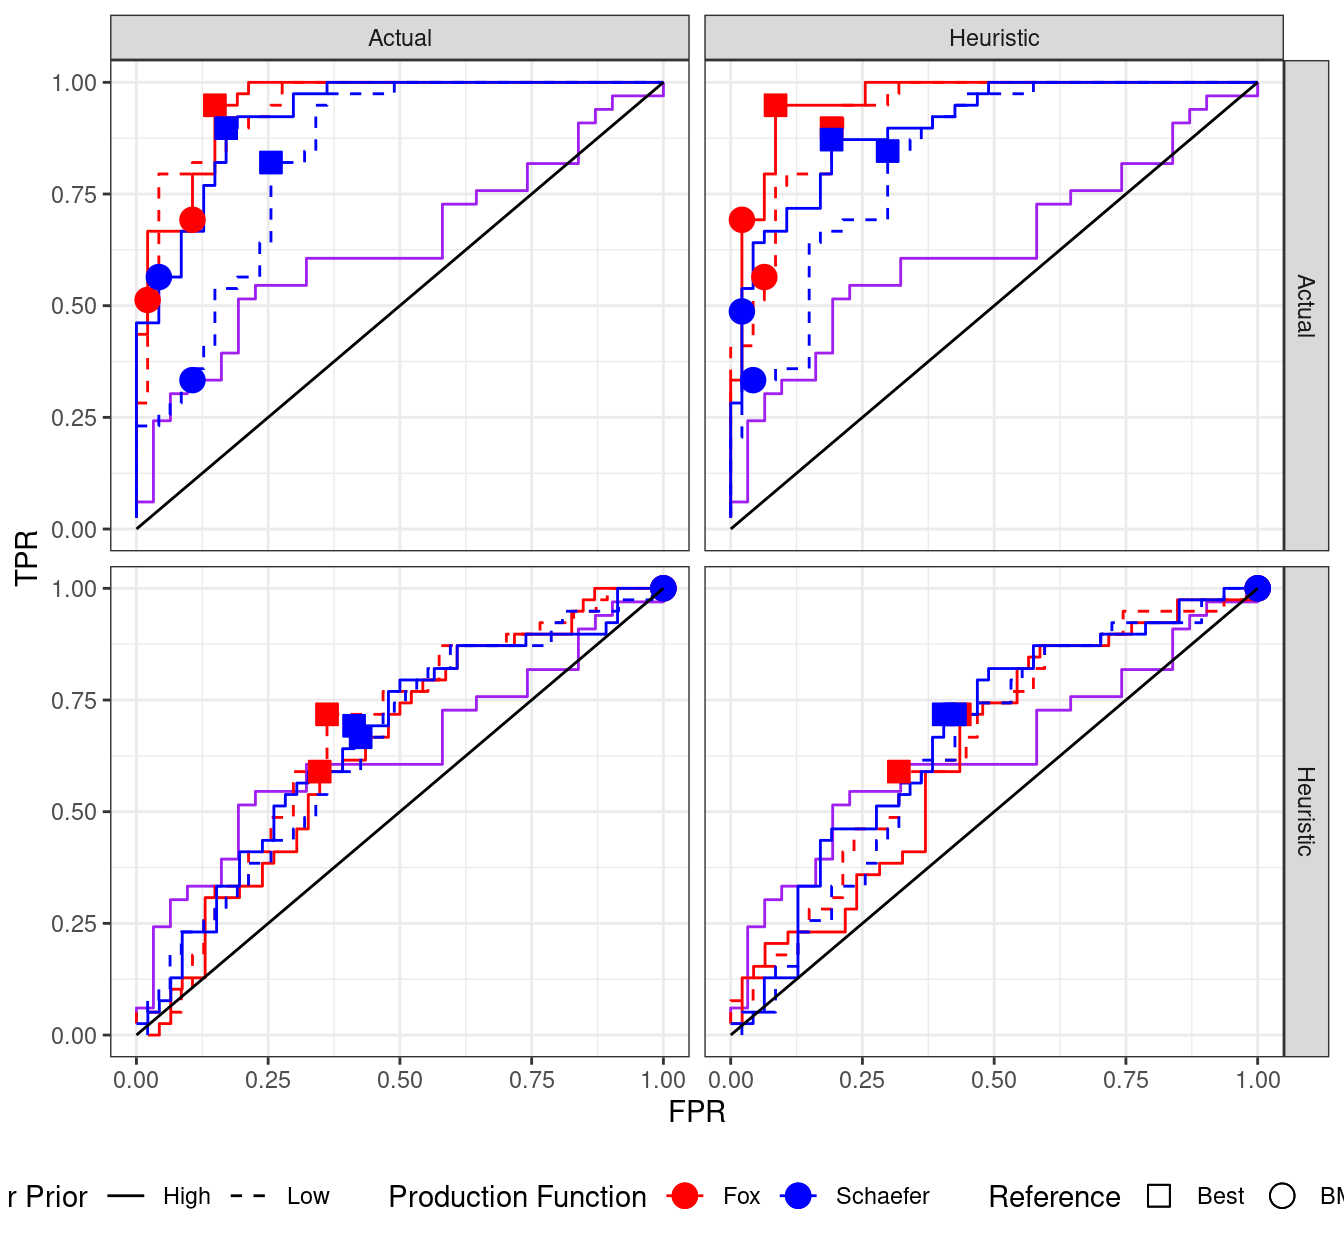
\includegraphics[width=0.75\textwidth]{figs/roc-1.png}
\caption{ROC curves for COMs.}
\label{fig:roc}
\end{figure}
